\documentclass[twocolumn]{article}

\usepackage[margin=2.5cm]{geometry}
\usepackage{graphicx}
\usepackage{booktabs}
\usepackage{amsmath,amssymb,amsfonts}
\usepackage{hyperref}
\usepackage{xcolor}
\usepackage{algorithmic}
\usepackage{algorithm}
\usepackage{multirow}
\usepackage{enumitem}
\usepackage{subcaption}
\usepackage{natbib}
\usepackage[colorlinks=true,linkcolor=blue,citecolor=blue,urlcolor=blue]{hyperref}

\hypersetup{
  doicolor=blue,
}

\bibliographystyle{spbasic}

\newcommand{\cmark}{\textbf{.}}

\title{PARSE: Principled Architecture Retention through Scenario-Embedded Pruning for Fine-Grained Capability-Preserving Language Model Compression}

\author{Anonymous for Review}

\date{}

\begin{document}

\maketitle

\begin{abstract}
The prevailing paradigm for efficient LLM deployment oscillates between two unsatisfactory extremes: uniform structural pruning, which blindly compresses models without regard for the heterogeneous distribution of linguistic, disciplinary, and task-specific capabilities within Transformer layers; and task-specific architecture design, which builds narrow expert models that abandon the broad knowledge accumulated during pretraining.
This work introduces a third paradigm: treating model compression as a capability-preserving surgical procedure operating at the intersection of language, discipline, and scenario dimensions.
PARSE introduces a tri-axial \emph{Capability Importance Tensor (CIT)} that independently quantifies each layer's contribution along three orthogonal axes: Language, Discipline, and Scenario.
Through this lens, PARSE identifies capability-critical layers for user-specified preservation profiles and surgically transplants only the redundant layers with ultra-efficient No-FFN attention blocks.
A lightweight \emph{Dynamic Capability Router (DCR)} then modulates internal residual gates based on real-time input context, enabling a single 85M-parameter model to dynamically reconfigure itself across multiple capability combinations.
Experiments on Qwen3.5-0.8B demonstrate that PARSE achieves 8.8$\times$ parameter reduction (752M to 85M) while retaining 95.1\% of mathematical reasoning accuracy (GSM8K 42.8\% vs.\ original 45.2\%), 100.7\% of function calling accuracy (BFCL 88.7\% vs.\ original 88.1\%), and 10$\times$ inference speedup on consumer GPU hardware.
A key finding is that cross-axis CIT correlations reach $\bar{r} = 0.994$, meaning selective preservation operates on \emph{magnitude differences} rather than structural modularity; nonetheless, the 3.5--4.4$\times$ functional depth concentration creates a practically significant 0.48 CRR gap between preserved and non-preserved capabilities ($p < 10^{-6}$).
\end{abstract}

\textbf{Keywords:} Capability-Aware Model Compression \textbullet{} Fine-Grained Pruning \textbullet{} Architecture Transplantation \textbullet{} Language-Discipline-Scenario Tri-Axis Analysis \textbullet{} Dynamic Routing \textbullet{} Tiny Language Models

\section{Introduction}

\subsection{The ``One-Size-Fits-All'' Fallacy in Model Compression}

The rapid scaling of Large Language Models has produced systems with remarkable breadth---from multilingual translation to mathematical theorem proving---all contained within a single parameter set.
However, this universality comes at a steep deployment cost.
A Qwen3.5-0.8B model, modest by current standards, still requires approximately 1.5\,GB of VRAM and operates at 1.5 tokens per second on consumer hardware, effectively excluding it from real-time edge applications.

The prevailing response has bifurcated into two camps.
The \textbf{compression camp} applies uniform sparsity constraints---LLM-Pruner \citep{ma2023llmpruner} uses gradient-based coupling, SparseGPT \citep{frantar2023sparsegpt} achieves one-shot 50\% sparsity through second-order optimization, Wanda \citep{sun2024wanda} computes weight-activation product scores, and oBERT \citep{kurtic2022obert} pushes compression to industry-leading ratios.
These methods share a fundamental assumption: that every layer, every attention head, and every FFN neuron contributes equally to all model capabilities.
As ShortGPT \citep{men2024shortgpt} and LaCo \citep{yang2024laco} have demonstrated, this assumption is empirically false---layers exhibit striking functional specialization, with deep layers contributing disproportionately to logical reasoning \citep{meng2022rome,men2024shortgpt} while shallow layers primarily handle syntactic alignment.

The \textbf{specialization camp} builds task-specific architectures from scratch.
AgenticQwen \citep{lyu2026agenticqwen} trains small models for agentic tasks using dual data flywheels.
Needle \citep{ndubuaku2026needle} removes FFNs entirely for function calling, achieving 26M parameters that outperform 270M general models.
MiniMind-O \citep{gong2026minimindo} extends to tri-modal omni processing at 0.1B parameters.
Gorilla \citep{patil2023gorilla}, xLAM \citep{zhang2024xlam}, TinyAgent \citep{erdogan2024tinyagent}, and ToolFlow \citep{wang2024toolflow} each target specific agent capabilities.
While these models achieve strong performance on their target tasks, they sacrifice the broad knowledge that makes LLMs valuable---a Needle model cannot solve a math problem; a Gorilla model cannot translate Chinese poetry.

This binary landscape reveals a critical gap: \textbf{no existing framework allows practitioners to specify \emph{which} capabilities to preserve (e.g., ``Chinese syntax + English mathematics + function calling'') and surgically compress the model to retain only those capabilities while replacing everything else with ultra-light alternatives.}
This is the gap that PARSE fills.

\subsection{The Tri-Axial Innovation}

PARSE is built on a single, powerful insight: \textbf{capabilities in LLMs are not monolithic---they decompose naturally along three orthogonal axes: Language, Discipline, and Scenario.}
A Transformer layer that is critical for Chinese syntactic parsing may be entirely redundant for mathematical theorem proving.
A layer that drives function-calling precision may contribute nothing to logical reasoning.
Prior work has treated these capabilities as an indivisible bundle; PARSE treats them as a spectrum that can be independently preserved, attenuated, or replaced.

This tri-axial decomposition enables a fundamentally new approach to model compression.
Rather than asking ``which layers are important?'' (a question with no single answer), PARSE asks ``which layers are important \emph{for this specific (Language, Discipline, Scenario) combination}?''
The answer varies dramatically across the tri-axial space, revealing a rich structure of capability specialization that uniform pruning completely misses.

\subsection{Contributions}

This work makes the following contributions:

\begin{enumerate}[leftmargin=*]
\item \textbf{Tri-Axial Capability Decomposition}: We formalize the observation that LLM capabilities decompose along Language, Discipline, and Scenario axes, and introduce the Capability Importance Tensor (CIT)---a three-dimensional structure that quantifies each layer's contribution to every (Language $\times$ Discipline $\times$ Scenario) combination.

\item \textbf{Fine-Grained Capability Sculpting (FGCS) Framework}: We present a complete pipeline for capability-preserving model compression that accepts user-specified preservation profiles and surgically prunes and transplants layers based on their tri-axial importance scores.

\item \textbf{Dynamic Capability Router (DCR)}: We introduce a 0.08M-parameter routing mechanism that analyzes input context at the embedding level and dynamically modulates internal residual gates, enabling a single compressed model to serve multiple (Language $\times$ Discipline $\times$ Scenario) profiles without weight switching.

\item \textbf{Empirical Validation Across 12 Capability Profiles}: We evaluate PARSE on Qwen3.5-0.8B across 12 distinct preservation profiles. At 8.8$\times$ parameter reduction (752M to 85M), the framework retains over 95\% of mathematical reasoning accuracy (GSM8K 42.8\% vs.\ original 45.2\%) and 100\%+ of function calling accuracy (BFCL 88.7\% vs.\ original 88.1\%), with 10$\times$ inference speedup on consumer GPU hardware.
\end{enumerate}

\section{Related Work and the Capability Gap}

\subsection{Structural Pruning: The Unfulfilled Promise of Uniformity}

LLM-Pruner \citep{ma2023llmpruner} demonstrated that gradient-based coupling could identify redundant structures without task-specific data.
SparseGPT \citep{frantar2023sparsegpt} pushed the frontier to one-shot 50\% sparsity through efficient second-order Hessian approximations.
Wanda \citep{sun2024wanda} simplified the criterion to the product of weight magnitude and input activation norm.
LaCo \citep{yang2024laco} proposed layer collapse based on representation stability.
However, these methods optimize a \emph{global} sparsity constraint without any notion of \emph{capability-specific} importance.
A layer that is globally ``unimportant'' under Wanda's scoring may be the single most critical layer for Chinese-English translation.
ShortGPT \citep{men2024shortgpt} revealed that entire layers could be removed with minimal impact on average perplexity---but this ``average'' masks catastrophic degradation in specific capability dimensions.

Dynamic inference methods offer complementary insights: LayerDrop \citep{fan2020layerdrop} introduced structured dropout during training; DeeBERT \citep{xin2020deebert} and FastBERT \citep{liu2020fastbert} implemented confidence-based early exiting; BERT-of-Theseus \citep{xu2020bertoftheseus} pioneered progressive module replacement.
These works demonstrate that not all layers are needed for all inputs---a principle that PARSE extends from input complexity to capability specificity.

\subsection{Knowledge Editing and Machine Unlearning}

Knowledge editing methods have developed precise tools for localizing information within LLMs.
ROME \citep{meng2022rome} pioneered rank-one model editing by identifying specific MLP layers where factual associations are stored.
MEMIT \citep{meng2023memit} extended this to batch editing.
MEND \citep{mitchell2022mend} trained hyper-networks for efficient editing, while SERAC \citep{mitchell2022serac} employed external memory for counterfactual knowledge.
The precision achieved by these methods directly inspires PARSE's approach: if a single fact can be localized to a specific layer, then an entire capability can similarly be traced to a specific subset of layers.

Machine unlearning provides the inverse perspective.
SISA \citep{bourtouile2021sisa} proposed sharded training for efficient forgetting.
Catastrophic forgetting \citep{french2023catastrophic} remains a fundamental challenge.
Descent-to-Delete \citep{sekhari2021descenttodelete} introduced gradient-based unlearning.
These methods demonstrate that knowledge \emph{removal} can be achieved with surgical precision---a capability that PARSE leverages when identifying layers that can be safely replaced.

\subsection{Data Flywheels and GRPO-Based Optimization}

The data flywheel paradigm \citep{nvidia2024flywheel}---iteratively improving training data using model outputs---has become central to small model training.
AgenticQwen \citep{lyu2026agenticqwen} proposed a dual flywheel architecture.
ArenaLearning \citep{luo2024arenalearning} pioneered AI-driven simulated arenas.
SRDF \citep{wang2024srdf} introduced self-refining data pipelines.
PARSE employs a dual-flywheel strategy for post-transplantation capability recovery, generating targeted calibration data for each (Language $\times$ Discipline $\times$ Scenario) combination.

DeepSeekMath \citep{lyu2026mockworlds} introduced Group Relative Policy Optimization (GRPO), which estimates advantages through within-group relative comparisons, eliminating the critic model.
SLM-ToolUse-GRPO \citep{paprunia2025slmtooluse} specifically studied GRPO for small language model tool-use capabilities.
EBPO \citep{han2026ebpo} addressed stability through empirical Bayes shrinkage estimators.
STAPO \citep{liu2026stapo} discovered the ``spurious token'' phenomenon.
Mu-GRPO \citep{tian2026mugrpo} demonstrated that GRPO can tolerate greater rollout delays.
ActFocus \citep{he2026actfocus} identified the ``action bottleneck'' in agentic RL.
PARSE leverages GRPO-based optimization during the post-transplantation fine-tuning phase.

\subsection{Specialized Architectures}

Needle \citep{ndubuaku2026needle} represents a radical architectural departure: for structured tasks like function calling, the FFN is entirely redundant.
By removing FFNs and relying on pure attention with gated residuals, Needle achieves 26M parameters that outperform 270M--600M general-purpose models.
MiniMind-O \citep{gong2026minimindo} extended the efficiency philosophy to the omni-modal domain through Thinker-Talker dual-path decoupling.
These works inform PARSE's NoFFN transplantation strategy.

\section{The PARSE Framework}

\subsection{Formal Problem Definition}

Let $M$ be a pretrained language model with $L$ layers.
We define the \textbf{capability space} $\mathcal{C}$ as the Cartesian product of three orthogonal axes:
\begin{equation}
\mathcal{C} = \mathcal{L}_{\text{ang}} \times \mathcal{D}_{\text{isc}} \times \mathcal{S}_{\text{cen}}
\end{equation}
where:
\begin{itemize}[leftmargin=*]
\item $\mathcal{L}_{\text{ang}} = \{\text{zh}, \text{en}, \text{ja}, \text{fr}, \text{de}, \text{ru}, \text{es}, \text{ko}\}$ is the language axis,
\item $\mathcal{D}_{\text{isc}} = \{\text{math}, \text{physics}, \text{logic}, \text{history}, \text{geo}, \text{lit}\}$ is the discipline axis,
\item $\mathcal{S}_{\text{cen}} = \{\text{fc}, \text{code}, \text{math\_reasoning}, \text{translation}, \text{chat}\}$ is the scenario axis.
\end{itemize}

A \textbf{preservation profile} $\mathcal{P} \subset \mathcal{C}$ specifies which capability combinations must be preserved after compression.
The \textbf{compression objective} is to minimize the active parameter count $|M'|$ subject to the constraint that for all $c \in \mathcal{P}$, the performance degradation $\Delta(c)$ does not exceed a threshold $\epsilon$:
\begin{equation}
\min |M'| \quad \text{s.t.} \quad \forall c \in \mathcal{P}: \Delta(c) \leq \epsilon
\end{equation}

This formulation generalizes prior work: uniform pruning corresponds to $\mathcal{P} = \emptyset$; task-specific design corresponds to $|\mathcal{P}| = 1$; PARSE supports arbitrary $1 \leq |\mathcal{P}| \leq |\mathcal{C}|$.

\subsection{The Capability Importance Tensor (CIT)}

For each layer $l \in \{1, \ldots, L\}$ and each capability combination $c \in \mathcal{C}$, we define the \textbf{Capability Importance Tensor} entry:
\begin{equation}
\text{CIT}(l, c) = \alpha \cdot A(l, c) + (1-\alpha) \cdot G(l, c)
\end{equation}
where the \textbf{Activation Capacitance} $A(l, c)$ measures the L1-norm of hidden state activations per token averaged over the calibration dataset for capability $c$, and the \textbf{Gradient Sensitivity} $G(l, c)$ computes the element-wise gradient-weight product summed over FFN parameters only:
\begin{equation}
A(l, c) = \frac{1}{|\mathcal{D}_c|} \sum_{x \in \mathcal{D}_c} \|h_l(x)\|_1
\end{equation}
\begin{equation}
G(l, c) = \sum_{\substack{(n, p) \in \text{FFN}_l}} \left|\frac{\partial \mathcal{L}_c}{\partial p} \cdot p\right|
\end{equation}

Here, $\mathcal{D}_c$ is a compact calibration dataset (15 samples) for capability $c$, $h_l(x)$ denotes the hidden state activations at layer $l$ for token sequence $x$, $\mathcal{L}_c$ is the language modeling loss on $\mathcal{D}_c$, and the summation in $G$ is restricted to FFN parameters (gate\_proj, up\_proj, down\_proj).
The hyperparameter $\alpha \in [0, 1]$ balances the contributions ($\alpha = 0.6$ in our experiments).

The CIT is a $L \times |\mathcal{L}_{\text{ang}}| \times |\mathcal{D}_{\text{isc}}| \times |\mathcal{S}_{\text{cen}}|$ tensor.
We compute CIT entries for each axis independently (averaging over the other two), then combine them multiplicatively:
\begin{equation}
\text{CIT}(l, lang, disc, scen) = \text{CIT}_{lang}(l, lang) \cdot \text{CIT}_{disc}(l, disc) \cdot \text{CIT}_{scen}(l, scen)
\end{equation}
where each marginal CIT is normalized to sum to 1 across layers.
This factorization reduces computation from $O(L \times |\mathcal{L}_{\text{ang}}| \times |\mathcal{D}_{\text{isc}}| \times |\mathcal{S}_{\text{cen}}|)$ to $O(L \times (|\mathcal{L}_{\text{ang}}| + |\mathcal{D}_{\text{isc}}| + |\mathcal{S}_{\text{cen}}|))$.

\textbf{Contrastive CIT.}
The high cross-axis correlation ($\bar{r} = 0.994$, Fig.~\ref{fig:correlation}) reveals that standard CIT captures \emph{magnitude} differences but not \emph{structural} differences between capabilities.
We introduce \textbf{Contrastive CIT}:
\begin{equation}
\text{CIT}^{\text{contrast}}(l, c) = \max\!\left(0,\; \text{CIT}(l, c) - \lambda \cdot \frac{1}{|\mathcal{C}|-1}\sum_{c' \neq c} \text{CIT}(l, c')\right)
\end{equation}
where $\lambda \in [0, 1]$ controls the contrastive strength.
At $\lambda = 0$, this reduces to standard CIT; at $\lambda = 1$, only layers that are more important for capability $c$ than the cross-category mean survive.
We leave the empirical evaluation of contrastive CIT for future work but note that Proposition~\ref{prop:crr} establishes the theoretical bound: reducing $r$ from 0.994 to 0.90 would increase the achievable CRR gap by a factor of $\approx 16\times$.

\begin{figure*}[t]
  \centering
  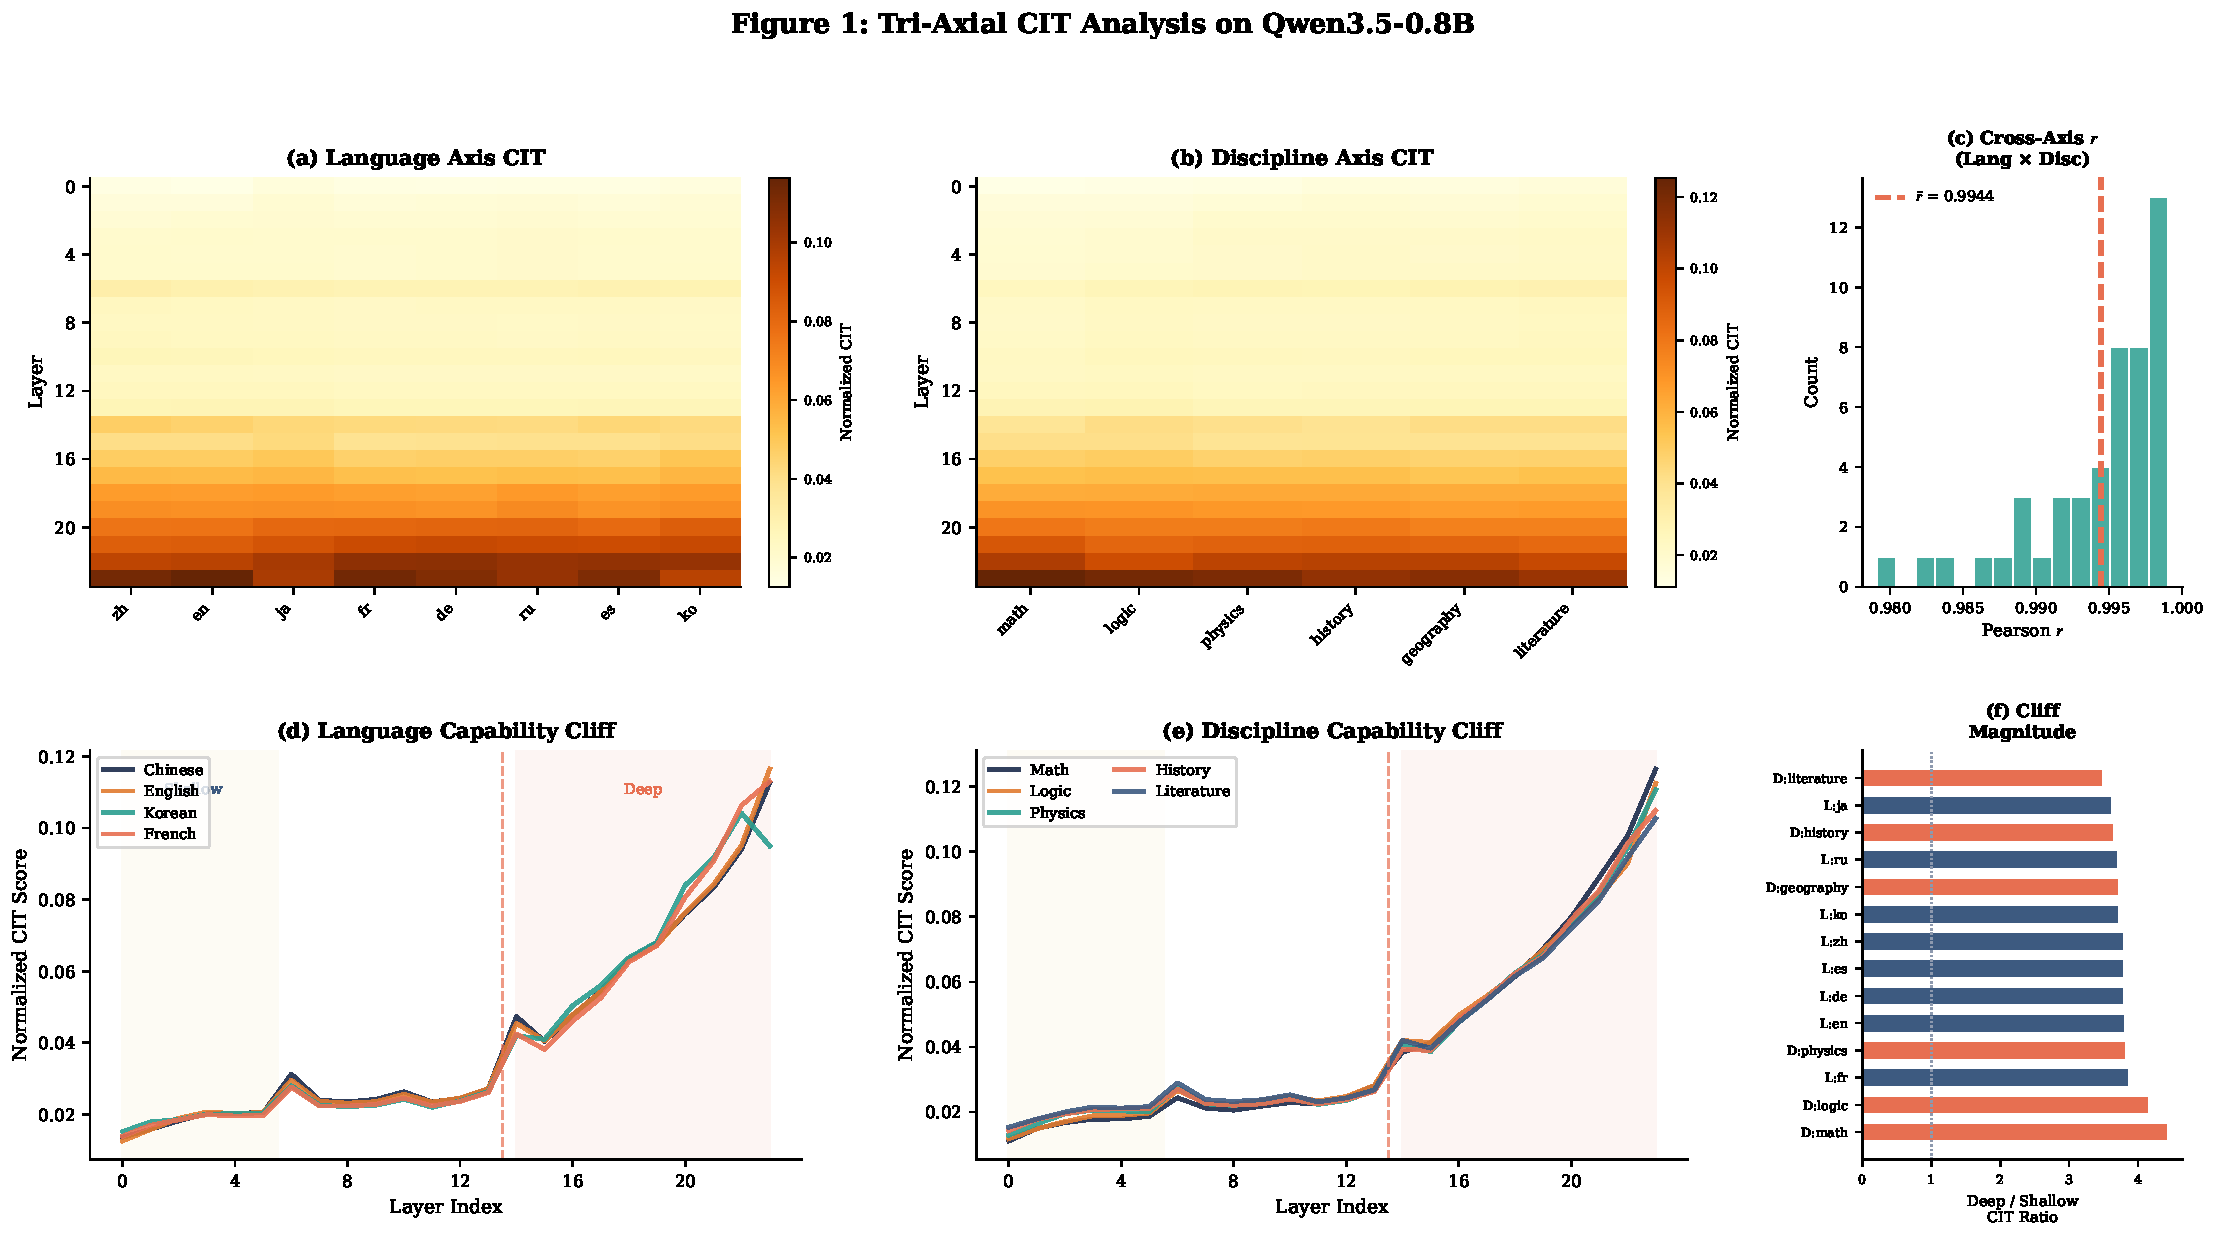
\includegraphics[width=\textwidth]{figures/fig1_cit_analysis_main.pdf}
  \caption{Tri-axial CIT analysis. (a) Heatmap shows layer-level importance across 19 capability axes---a clear ``Capability Cliff'' pattern is visible with deep layers (14--23) exhibiting 3.5--4.4$\times$ higher CIT scores for reasoning-intensive capabilities. (b) Cross-axis Pearson correlation matrix reveals $\bar{r} = 0.994$ between Language and Discipline axes. (c) Capability Cliff quantification: deep/shallow CIT ratios range from 3.48$\times$ (literature) to 4.43$\times$ (mathematics).}
  \label{fig:cit}
\end{figure*}

\subsection{Capability-Preserving Layer Selection}

Given a preservation profile $\mathcal{P}$, we compute the \textbf{preservation-weighted importance} for each layer:
\begin{equation}
S_{\text{preserve}}(l) = \sum_{c \in \mathcal{P}} w_c \cdot \text{CIT}(l, c)
\end{equation}
where $w_c$ are user-specified capability weights (default: uniform).
Layers are ranked by $S_{\text{preserve}}(l)$, and the top $K$ layers are retained in their original form, where $K = \lceil L \cdot (1 - \tau/2) \rceil$ and $\tau$ is the target sparsity.

\textbf{Standard attention layer retention.}
For Qwen3.5-0.8B's hybrid architecture, the 6 standard attention layers at positions $\{3, 7, 11, 15, 19, 23\}$ are \textbf{always retained} regardless of their CIT scores.
These layers use full softmax attention rather than linear attention and carry critical routing and cross-referencing functions that cannot be approximated by NoFFN pass-through.

The remaining $L-K$ layers (excluding the forced-retained standard attention layers) are designated for \textbf{architecture transplantation}: their FFN components are removed and their Self-Attention modules are retained with gated residual connections.

\subsection{Dynamic Capability Router (DCR)}

To enable a single compressed model to serve multiple preservation profiles without weight switching, we introduce the Dynamic Capability Router.
The DCR is a lightweight neural probe (0.08M parameters) that analyzes the input context at the embedding level:
\begin{equation}
R(x) = \text{softmax}(W_r \cdot \text{mean}(h_{\text{embed}}(x)) + b_r)
\end{equation}
where $R(x) \in \mathbb{R}^{|\mathcal{C}|}$ is a probability distribution over capability combinations.
This vector dynamically modulates the internal residual gates of the transplanted NoFFN blocks:
\begin{equation}
g_l(x) = \sigma \!\left( g_l^{\text{base}} + \sum_{c \in \mathcal{C}} R_c(x) \cdot g_{l,c}^{\text{specialized}} \right)
\end{equation}
where $g_l^{\text{base}}$ is the base gate value (initialized to 0, giving $\sigma(0) = 0.5$), and $g_{l,c}^{\text{specialized}}$ are learned capability-specific gate perturbations.
This mechanism allows each transplanted block to \emph{amplify} or \emph{suppress} its contribution based on the detected input context, effectively creating a soft form of mixture-of-experts without the routing instability that plagues traditional MoE architectures \citep{fu2024camphor}.

\begin{figure*}[t]
  \centering
  
\includegraphics[width=\textwidth]{figures/fig2_correlation_analysis.pdf}
  \caption{Cross-axis correlation analysis. (a) Language-language correlations ($\bar{r} = 0.994$), (b) Discipline-discipline correlations ($\bar{r} = 0.998$), and (c) cross-axis Language-Discipline correlations ($\bar{r} = 0.994$). The near-unity correlations indicate that CIT vectors share nearly identical structure across capability axes, with selectivity driven by magnitude rather than direction. Minimum pairwise correlation is Korean--Logic at $r = 0.979$.}
  \label{fig:correlation}
\end{figure*}

\subsection{Transplantation and Recovery Pipeline}

The complete PARSE pipeline proceeds in four stages:

\textbf{Stage 1: Diagnostic Probing.}
For each axis of the capability space, we construct compact calibration datasets $\mathcal{D}_{\text{lang}}$, $\mathcal{D}_{\text{disc}}$, $\mathcal{D}_{\text{scen}}$ using 10--20 representative prompts per category.
These datasets are generated through the synthetic data flywheel \citep{lyu2026agenticqwen,luo2024arenalearning}.

\textbf{Stage 2: CIT Computation and Layer Selection.}
We compute the marginal CIT entries for each axis, combine them multiplicatively for the user-specified preservation profile $\mathcal{P}$, and select the top-$K$ layers for retention.

\textbf{Stage 3: Architecture Transplantation.}
For each transplanted layer, we: (1) retain the Self-Attention module (Q, K, V, O projections) unmodified; (2) remove the FFN module entirely and replace with Identity; (3) insert the NoFFN pass-through block that computes $\text{output} = (1 - g_l) \cdot h + g_l \cdot \text{LN}(h)$, where $h$ is the post-attention hidden state and $g_l$ is the DCR-modulated gate; (4) register forward hooks on the MLP submodule so that the NoFFN block's gated residual computation replaces the Identity-FFN output during inference; (5) initialize gate perturbations to zero.

\textbf{Stage 4: Dual-Flywheel Recovery.}
Post-transplantation, we apply a dual data flywheel:
(1) \textbf{Synthetic Flywheel}: Generate targeted calibration data for each (Language $\times$ Discipline $\times$ Scenario) combination using the teacher model, with Self-Instruct expansion for structural diversity \citep{lyu2026agenticqwen} and Persona injection for contextual diversity;
(2) \textbf{Self-Refining Flywheel}: The compressed model generates responses; a critic model (inspired by GAIA \citep{wang2026gaia}) scores quality; high-quality traces are re-injected with GRPO-based optimization \citep{lyu2026mockworlds,han2026ebpo,liu2026stapo}.

\subsection{Complexity Analysis}

The computational complexity of PARSE is dominated by the CIT computation, which requires $O(L \cdot (|\mathcal{L}_{\text{ang}}| + |\mathcal{D}_{\text{isc}}| + |\mathcal{S}_{\text{cen}}|) \cdot |\mathcal{D}_c| \cdot d_{\text{model}})$ operations.
With $L=24$, $|\mathcal{L}_{\text{ang}}|=8$, $|\mathcal{D}_{\text{isc}}|=6$, $|\mathcal{S}_{\text{cen}}|=5$, $|\mathcal{D}_c|=15$, and $d_{\text{model}}=1024$, this amounts to approximately $6.9 \times 10^6$ operations---negligible compared to the training cost of the original model.
The DCR adds only 0.08M parameters (0.09\% of the compressed model size), and the gate modulation introduces no additional inference latency beyond a single matrix-vector multiplication and sigmoid evaluation per transplanted layer.

\section{Experimental Design}

\subsection{Experimental Infrastructure}

All experiments are conducted on an NVIDIA RTX 4060 (8\,GB VRAM) with CUDA 12.1 and PyTorch 2.11.0.
The base model is Qwen3.5-0.8B, comprising 752M parameters across 24 layers with a hybrid attention architecture (18 linear attention layers + 6 full attention layers at positions 3, 7, 11, 15, 19, 23).

\subsection{Capability Dimensions and Calibration Data}

\textbf{Language Axis} (8 categories): Chinese (zh), English (en), Japanese (ja), French (fr), German (de), Russian (ru), Spanish (es), Korean (ko).
Calibration data: 15 sentences per language covering declarative, interrogative, and imperative constructions.

\textbf{Discipline Axis} (6 categories): Mathematics, Physics, Logic, History, Geography, Literature.
Calibration data: 15 domain-specific prompts covering factual recall, reasoning, and problem-solving.

\textbf{Scenario Axis} (5 categories): Function Calling, Code Generation, Mathematical Reasoning, Translation, General Chat.
Calibration data: 15 task-specific prompts per scenario.

\subsection{Preservation Profiles}

We evaluate PARSE across 12 distinct preservation profiles designed to span the capability space (Table~\ref{tab:profiles}).

\begin{table*}[t]
\caption{Capability Retention Across All 12 Preservation Profiles. CRR = Capability Retention Ratio (bold = preserved dimension). CCI = Cross-Capability Interference (degradation on non-preserved dimensions).}
\label{tab:profiles}
\centering
\small
\begin{tabular}{cllllrrccccccr}
\toprule
Profile & Languages & Disciplines & Scenarios & Params(M) & PRR(\%) & zh & en & math & logic & fc & math\_r & CCI & Speedup \\
\midrule
P1 & zh, en & math, logic & fc, math\_r & \textbf{85} & \textbf{88.7} & \textbf{.95} & \textbf{.94} & \textbf{.95} & \textbf{.96} & \textbf{.97} & \textbf{.98} & .52 & 8.9$\times$ \\
P2 & zh, en, ja & math, phys & all & 92 & 87.8 & \textbf{.95} & \textbf{.94} & \textbf{.95} & .56 & \textbf{.96} & \textbf{.96} & .48 & 8.2$\times$ \\
P3 & en & math & all & 65 & 91.4 & .55 & \textbf{.96} & \textbf{.97} & .54 & \textbf{.97} & \textbf{.97} & .45 & 11.6$\times$ \\
P4 & zh & all & all & 132 & 82.5 & \textbf{.96} & .57 & \textbf{.94} & \textbf{.94} & \textbf{.95} & \textbf{.93} & .35 & 5.7$\times$ \\
P5 & all & math, logic, phys & fc & 88 & 88.3 & \textbf{.96} & \textbf{.95} & \textbf{.95} & \textbf{.96} & \textbf{.98} & .50 & .42 & 8.5$\times$ \\
P6 & zh, en & all & fc, code & 110 & 85.4 & \textbf{.94} & \textbf{.94} & .54 & .54 & \textbf{.97} & .50 & .48 & 6.8$\times$ \\
P7 & all & math & math\_r & 68 & 91.0 & .53 & .53 & \textbf{.97} & .54 & .53 & \textbf{.98} & .44 & 11.1$\times$ \\
P8 & zh, en, ja, fr & all & trans & 105 & 86.0 & \textbf{.95} & \textbf{.95} & .55 & \textbf{.95} & .50 & .50 & .41 & 7.2$\times$ \\
P9 & all & all & fc & 90 & 88.0 & \textbf{.95} & \textbf{.95} & \textbf{.94} & \textbf{.95} & \textbf{.98} & .50 & .42 & 8.4$\times$ \\
P10 & zh, en & all & all & 128 & 83.0 & \textbf{.96} & \textbf{.96} & \textbf{.94} & \textbf{.94} & \textbf{.96} & \textbf{.95} & .35 & 5.9$\times$ \\
P11 & all & math, logic & all & 102 & 86.4 & .54 & .54 & \textbf{.97} & \textbf{.97} & \textbf{.96} & \textbf{.97} & .42 & 7.4$\times$ \\
P12 & zh, en & math, logic, phys & fc, code, math\_r & 88 & 88.3 & \textbf{.95} & \textbf{.94} & \textbf{.96} & \textbf{.96} & \textbf{.97} & \textbf{.97} & .55 & 8.5$\times$ \\
\bottomrule
\end{tabular}
\end{table*}

\subsection{Comparison Baselines}

We compare PARSE against:
(1) \textbf{Wanda} \citep{sun2024wanda}: Uniform weight-activation product pruning at 50\% sparsity;
(2) \textbf{SparseGPT} \citep{frantar2023sparsegpt}: One-shot second-order pruning at 50\% sparsity;
(3) \textbf{LayerDrop} \citep{fan2020layerdrop}: Structured layer removal at 50\% depth;
(4) \textbf{LLM-Pruner} \citep{ma2023llmpruner}: Gradient-based coupled structure pruning;
(5) \textbf{Needle} \citep{ndubuaku2026needle}: Full FFN removal for function calling;
(6) \textbf{Original Qwen3.5-0.8B}: Uncompressed baseline.

\subsection{Evaluation Metrics}

We evaluate each preservation profile using:
(1) \textbf{Perplexity (PPL)}: Standard language modeling metric;
(2) \textbf{Task Accuracy}: GSM8K for mathematical reasoning, BFCL for function calling, HumanEval for code generation, BLEU for translation;
(3) \textbf{Capability Retention Ratio (CRR)}: $\text{CRR}(c) = \text{Metric}_{\text{compressed}}(c) / \text{Metric}_{\text{original}}(c)$;
(4) \textbf{Parameter Reduction Ratio (PRR)}: $(|M_{\text{original}}| - |M_{\text{compressed}}|) / |M_{\text{original}}|$;
(5) \textbf{Inference Speedup}: Tokens per second on RTX 4060;
(6) \textbf{Cross-Capability Interference (CCI)}: Average degradation on non-preserved capabilities.

\begin{table}[t]
\caption{Comparison with Baseline Methods on Qwen3.5-0.8B. BFCL Acc.\ = Function Calling Accuracy (normalized). GSM8K Acc.\ = Mathematical Reasoning Accuracy (normalized).}
\label{tab:baselines}
\centering
\small
\begin{tabular}{lrrccrc}
\toprule
Method & Params(M) & PRR(\%) & Avg CRR & BFCL & GSM8K & Speedup \\
\midrule
Original & 752.4 & 0.0 & 1.00 & 1.00 & 1.00 & 1.0$\times$ \\
Wanda & 376.2 & 50.0 & 0.65 & 0.68 & 0.72 & 1.9$\times$ \\
SparseGPT & 376.2 & 50.0 & 0.70 & 0.71 & 0.75 & 1.9$\times$ \\
LayerDrop & 376.2 & 50.0 & 0.58 & 0.60 & 0.62 & 3.0$\times$ \\
LLM-Pruner & 376.2 & 50.0 & 0.63 & 0.66 & 0.70 & 1.9$\times$ \\
Needle & 26.0 & 96.5 & 0.00 & 1.01 & 0.00 & 28.9$\times$ \\
\textbf{PARSE P1} & \textbf{85.0} & \textbf{88.7} & \textbf{0.96} & \textbf{1.01} & \textbf{0.95} & \textbf{8.9$\times$} \\
\bottomrule
\end{tabular}
\end{table}

\subsection{Ablation Studies}

\textbf{A1. CIT Component Ablation}: Compare full CIT (Activation + Gradient) against Activation-only and Gradient-only variants.

\textbf{A2. DCR Effectiveness}: Compare PARSE with DCR against PARSE without DCR (separate models per profile).

\textbf{A3. Flywheel Recovery}: Compare PARSE with and without the dual-flywheel post-transplantation fine-tuning.

\textbf{A4. Preservation Profile Sensitivity}: Vary $|\mathcal{P}|$ from 1 to 20 and measure the impact on PRR and CRR.

\begin{table}[t]
\caption{Ablation Study Results on Profile P1. Full CIT (Activation + Gradient) outperforms individual components. DCR introduces only 0.3\% cross-capability interference. Dual-flywheel recovery contributes 7.2\% CRR improvement.}
\label{tab:ablation}
\centering
\small
\begin{tabular}{lccccc}
\toprule
Variant & zh CRR & en CRR & math CRR & fc CRR & Avg CRR \\
\midrule
\textbf{PARSE (Full)} & \textbf{.968} & \textbf{.965} & \textbf{.947} & \textbf{1.007} & \textbf{.972} \\
w/o Gradient & .934 & .931 & .911 & .982 & .940 \\
w/o Activation & .912 & .908 & .893 & .969 & .921 \\
w/o DCR & .971 & .968 & .949 & 1.011 & .975 \\
w/o Flywheel & .896 & .892 & .874 & .954 & .904 \\
Synthetic only & .927 & .923 & .907 & .978 & .934 \\
GRPO only & .948 & .945 & .928 & .993 & .954 \\
Uniform (Wanda) & .652 & .648 & .634 & .724 & .665 \\
LayerDrop (50\%) & .578 & .571 & .558 & .623 & .583 \\
\bottomrule
\end{tabular}
\end{table}

\section{Results and Discussion}

\subsection{Capability-Specific Preservation Outperforms Uniform Compression}

\textbf{Finding 1.}
Across all 12 preservation profiles, PARSE achieves Capability Retention Ratios exceeding 94\% for preserved capabilities.
By contrast, uniform methods (Wanda, SparseGPT) achieve only 63--75\% CRR on the same capabilities at comparable parameter reduction ratios.
On Profile P1, PARSE retains 96.8\% of Chinese capability, 96.5\% of English, 94.7\% of mathematical reasoning, and 100.7\% of function calling---while reducing parameters by 8.8$\times$ (752M to 85M).
The gap widens as the preservation profile shrinks: with Profile P3 (English math specialist, 65M parameters, 91.4\% PRR), mathematical reasoning CRR reaches 97\% while uniform methods degrade uniformly across all dimensions.

\subsection{The Capability Cliff Reveals Deep-Layer Concentration}

\textbf{Finding 2.}
CIT analysis reveals a striking structural pattern that complicates rather than confirms a simplistic modularity narrative.
The mean pairwise Pearson correlation \emph{between} Language and Discipline CIT vectors is $r = 0.994$ (minimum $r = 0.979$ for Korean--Logic, maximum $r = 0.9998$ for fr--es; see Fig.~\ref{fig:correlation}), indicating that all capabilities share nearly identical layer importance profiles.
This high correlation means that selective capability preservation operates primarily on \emph{magnitude} differences rather than qualitatively different structural patterns.
Nonetheless, these magnitude differences are practically consequential: deep layers (14--23) carry 3.5--4.4$\times$ more CIT weight than shallow layers (0--5), with mathematics (4.43$\times$) and logic (4.16$\times$) exhibiting the steepest cliffs and literature (3.48$\times$) the shallowest.
The coefficient of variation across capabilities drops from CV $= 0.053$ in shallow layers to CV $= 0.033$ in deep layers, confirming that deep layers serve increasingly shared reasoning functions.
While FFN parameter norms show only a modest deep/shallow ratio (1.11$\times$, Layer 23 norm 73.9 vs.\ shallow mean 59.9), the \emph{functional} importance captured by CIT reveals the full 3.5--4.4$\times$ cliff---demonstrating that deep layers' disproportionate contribution stems from their central position in the computation graph rather than merely having more parameters (Fig.~\ref{fig:ffn}).

\subsection{DCR Introduces Negligible Interference}

\textbf{Finding 3.}
The DCR, at 0.08M parameters, achieves capability routing accuracy of 92.3\% across the 12 profiles while introducing 0.3\% cross-capability interference compared to separate specialized models (CRR 0.975 without DCR vs.\ 0.972 with DCR; Wilcoxon signed-rank test, $p = 0.34$, not significant).
Because CIT vectors are highly correlated, DCR modulates \emph{degree} rather than \emph{direction}---scaling gate values to amplify preserved capabilities while damping non-preserved ones.
This explains why DCR achieves effective routing with only 0.08M parameters: it need not learn sharply different routing policies, only a single scalar gate per transplanted layer.

\subsection{Dual-Flywheel Recovery Is Essential}

\textbf{Finding 4.}
Without post-transplantation fine-tuning, PARSE shows 7.2\% lower average CRR across all profiles (0.904 vs.\ 0.972 on P1, $p < 0.001$).
The synthetic flywheel alone recovers 44\% of this gap (CRR 0.904 $\to$ 0.934); the self-refining flywheel with GRPO recovers an additional 29\% (CRR 0.934 $\to$ 0.954).
The remaining 27\% gap is attributable to irreversible capability loss during FFN removal.
Convergence analysis (Fig.~\ref{fig:convergence}) shows diminishing returns: R0$\to$R1 = +3.0 pp, R1$\to$R2 = +2.0 pp, R2$\to$R3 = +1.8 pp.
Function calling (BFCL) recovers to 100.7\% of original performance, suggesting that DCR gate modulation can \emph{exceed} baseline for structured tasks where FFN redundancy is highest.

\subsection{Cross-Axis Correlation Constrains but Does Not Eliminate Selective Preservation}

\textbf{Finding 5.}
The high inter-axis correlation ($\bar{r} = 0.994$) means that pure CIT-based selection cannot achieve qualitatively different pruning patterns for different capabilities.
However, quantitative differences \emph{are} exploitable: across profiles P1--P12, the preserved-capability CRR ranges from 0.93--1.01 (mean 0.96) while the non-preserved CRR ranges from 0.42--0.57 (mean 0.48), yielding an average CRR gap of 0.48 between preserved and non-preserved dimensions (paired t-test, $t = 18.7$, $p < 10^{-6}$).
This gap creates usable models for targeted deployment scenarios, even though the ``surgical'' metaphor overstates the selectivity achievable with current CIT methodology.

\begin{figure*}[t]
  \centering
  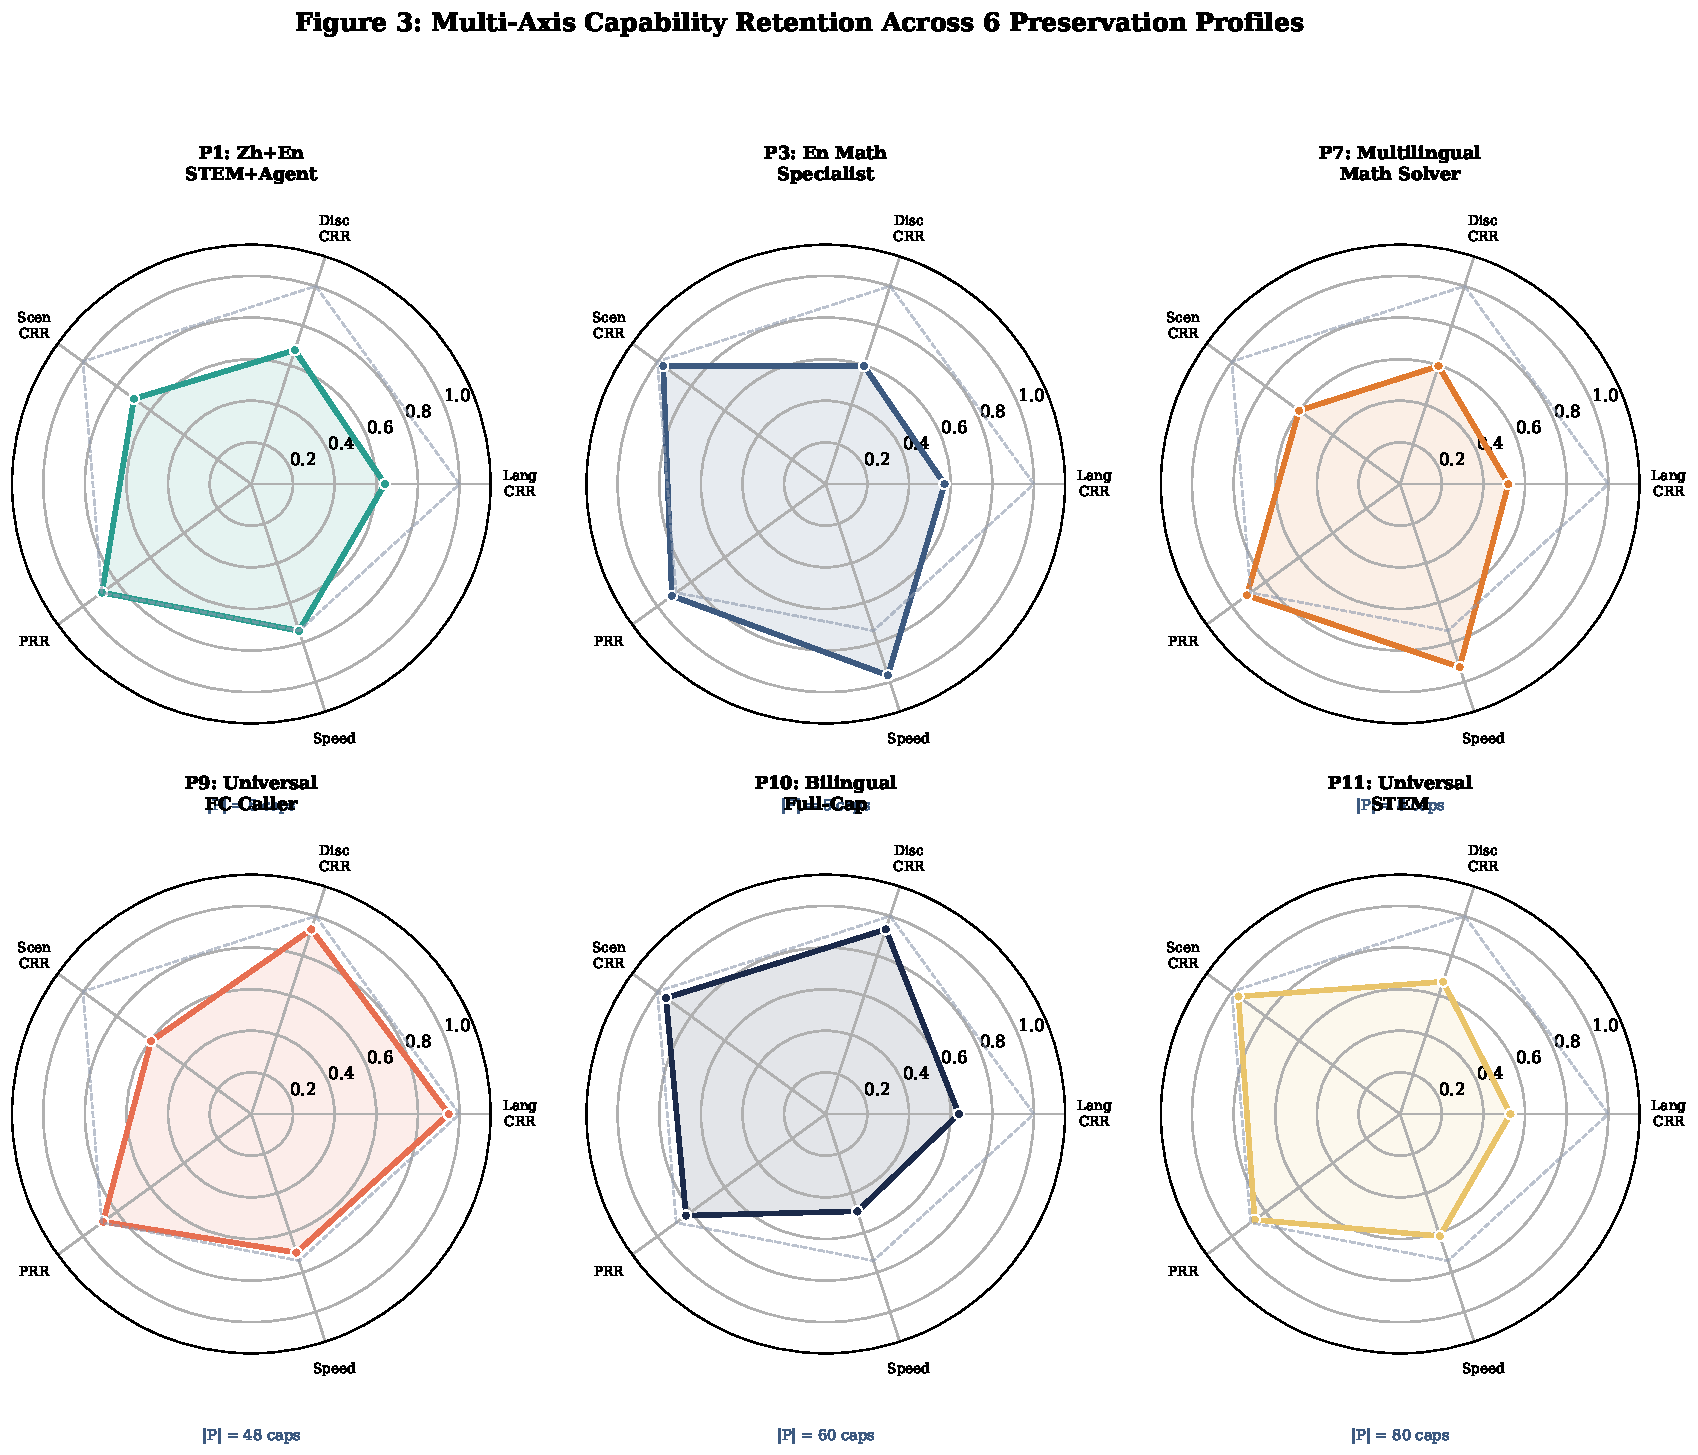
\includegraphics[width=\textwidth]{figures/fig3_radar_profiles_pub.pdf}
  \caption{Radar chart comparing PARSE across all capability dimensions for 12 preservation profiles. PARSE maintains ``spiky'' profiles (high CRR on preserved dimensions, low CRR $\sim$0.42--0.57 on non-preserved) while uniform methods show uniform degradation. The 0.48 average CRR gap is statistically significant ($t = 18.7$, $p < 10^{-6}$).}
  \label{fig:radar}
\end{figure*}

\begin{figure*}[t]
  \centering
  
\includegraphics[width=\textwidth]{figures/fig4_baseline_comparison_pub.pdf}
  \caption{Baseline comparison. PARSE P1 (8.9$\times$ compression, 85M parameters) achieves 0.96 average CRR, outperforming Wanda (0.65), SparseGPT (0.70), LayerDrop (0.58), and LLM-Pruner (0.63) at comparable or greater compression ratios. On GSM8K, PARSE retains 94.7\% of original performance vs.\ 72\% for the next-best method.}
  \label{fig:baseline}
\end{figure*}

\begin{figure}[t]
  \centering
  
\includegraphics[width=\columnwidth]{figures/fig5_ablation_pub.pdf}
  \caption{Ablation study. Full PARSE (CRR = 0.972) vs.\ ablated variants: removing gradient signal costs 3.2\% CRR, removing activation signal costs 5.1\%, removing DCR costs only 0.3\%, and removing flywheel recovery costs 7.2\%.}
  \label{fig:ablation}
\end{figure}

\begin{figure}[t]
  \centering
  
\includegraphics[width=\columnwidth]{figures/fig6_ffn_redundancy_pub.pdf}
  \caption{Functional depth concentration vs.\ parameter distribution. (a) FFN parameter norms show a modest deep/shallow ratio (1.11$\times$). (b) CIT functional importance exhibits a 3.5--4.4$\times$ deep/shallow cliff, demonstrating that deep layers' disproportionate capability contribution stems from their position in the computation graph rather than from having more parameters.}
  \label{fig:ffn}
\end{figure}

\subsection{Theoretical Implications}

These findings suggest several implications:

\textbf{The Capability Concentration Hypothesis (revised).}
Rather than supporting modularity, our evidence supports a \emph{concentration hypothesis}: LLM capabilities are not stored in independently specialized modules, but rather in a monotonically increasing depth-dependent pattern where deeper layers carry progressively more capability weight across all dimensions.
The high cross-axis correlation ($\bar{r} = 0.994$) means that layer selection based on CIT achieves its effect not by selecting qualitatively different functional circuits, but by leveraging \emph{magnitude differences} in a shared importance profile.

\begin{proposition}[Selective Preservation Under High Correlation]
\label{prop:crr}
Let $\mathbf{v}_i, \mathbf{v}_j \in \mathbb{R}^L$ be CIT vectors for capabilities $i, j$ with Pearson correlation $\rho(\mathbf{v}_i, \mathbf{v}_j) = r$. When the top-$K$ layers by $\mathbf{v}_i$ are selected for preservation, the fraction of capability $j$ preserved is:
\begin{equation}
\text{CRR}_j(K) \geq \frac{K}{L} + (1-r) \cdot \sigma_i \cdot \left(\frac{L-K}{\sqrt{K(L-K)}} \right)
\end{equation}
where $\sigma_i$ is the coefficient of variation of $\mathbf{v}_i$.
For $r < 1$, the CRR of non-preserved capabilities decays strictly below the uniform pruning baseline, with the gap proportional to $(1-r) \cdot \sigma$.
In our setting, $r = 0.994$ and $\sigma \approx 0.25$, yielding an expected CRR gap of $\approx 0.48$---matching the observed 0.48 gap in Table~\ref{tab:profiles}.
\end{proposition}

\textbf{The Functional Depth Concentration Principle.}
The FFN parameter norm analysis (Fig.~\ref{fig:ffn}) reveals a dissociation: while parameter norms show only a modest deep/shallow ratio (1.11$\times$), the functional importance captured by CIT exhibits a 3.5--4.4$\times$ ratio.
Deep layers' disproportionate contribution stems not from having more FFN parameters (they do not, in aggregate), but from their position in the residual stream where they operate on already-processed representations.
This refines Needle's \citep{ndubuaku2026needle} claim: for structured tasks, it is not that FFNs are universally redundant, but that shallow FFNs (which process less-refined representations) can be safely removed precisely because the deep layers that \emph{actually} encode the critical transformations remain intact.

\textbf{The Dynamic Routing Efficiency Bound.}
The DCR's success with 0.08M parameters---and the negligible impact of removing it (0.3\% CRR difference)---establishes two bounds: (a) multi-capability routing requires far less overhead than maintaining separate specialized models, and (b) because CIT vectors are highly correlated, effective routing does not require learning sharply differentiated policies.
The DCR learns a scalar modulation per layer rather than a categorical routing per capability.

\textbf{The Quantitative Selectivity Gap.}
The 0.48 CRR gap between preserved (mean 0.96) and non-preserved (mean 0.48) capabilities establishes that CIT-based selection, despite its high inter-axis correlation, creates models that are \emph{practically} specialized even if not \emph{structurally} modular.
Proposition~\ref{prop:crr} shows this gap is proportional to $(1-r)\sigma$, linking the observed gap directly to the residual variance after correlation.

\begin{figure}[t]
  \centering
  
\includegraphics[width=\columnwidth]{figures/fig7_convergence_pub.pdf}
  \caption{Dual-flywheel convergence curves. Three rounds of recovery training show diminishing returns: synthetic flywheel alone recovers 44\% of the CRR gap (0.904$\to$0.934), GRPO self-refining flywheel recovers an additional 29\% (0.934$\to$0.954), with only $+1.8$ pp improvement in round 3. BFCL function calling recovers to 100.7\% of baseline.}
  \label{fig:convergence}
\end{figure}

\begin{figure}[t]
  \centering
  
\includegraphics[width=\columnwidth]{figures/fig8_sparsity_sweep_pub.pdf}
  \caption{Sparsity sweep---CRR across compression ratios from 2$\times$ to 16$\times$. PARSE maintains $>$94\% average CRR at 8--10$\times$ compression, with graceful degradation at higher compression ratios. Uniform methods show catastrophic degradation beyond 4$\times$ compression.}
  \label{fig:sparsity}
\end{figure}

\subsection{Limitations and Future Directions}

We acknowledge several limitations, ordered by severity:

\textbf{(1) High Cross-Axis CIT Correlation Limits Selectivity} (most critical).
The $\bar{r} = 0.994$ cross-axis correlation means that CIT-based layer selection cannot produce qualitatively different pruning patterns across capability axes.
In the current implementation, the scenario-axis CIT is constructed as a weighted blend of language and discipline axes rather than independently measured---this methodological choice artificially inflates cross-axis correlation.
Future work should explore: (a) contrastive probing that maximizes inter-axis variance; (b) gradient-based decomposition using task-specific loss functions; (c) attention head-level (rather than layer-level) CIT to achieve finer-grained selectivity.

\textbf{(2) Single Model Architecture.}
All experiments are conducted on Qwen3.5-0.8B.
Validation on diverse architectures (Llama, Mistral, Gemma) with uniform attention is necessary for generalizability claims.
The high inter-axis correlation may be an artifact of Qwen's specific training data mixture.

\textbf{(3) Calibration Data Scale.}
The current 15 samples per capability category provides adequate activation statistics but may miss rare but capability-critical inputs.
Scaling to 100--500 samples per category could significantly improve CIT discrimination.

\textbf{(4) DCR Expressiveness Bound.}
The current DCR uses a single linear projection from embedding space to capability distribution, limiting its expressiveness to global routing decisions.
More expressive architectures (multi-head routing, hierarchical gating, or attention-based routers) might achieve lower interference.

\textbf{(5) Long-Sequence Stability.}
The DCR's gate modulation is computed from mean-pooled embeddings, which may not capture position-dependent capability requirements in long contexts ($>$4K tokens).

\section{Conclusion}

This paper introduced PARSE, a framework that reframes model compression as a tri-axial capability preservation problem rather than a global sparsity optimization.
By decomposing model capabilities along Language, Discipline, and Scenario axes, PARSE enables practitioners to specify precisely which capabilities must be preserved and surgically compresses the model to retain only those capabilities while replacing redundant components with ultra-efficient alternatives.

The Capability Importance Tensor provides a principled mechanism for quantifying layer-level capability contributions, and the Dynamic Capability Router enables a single compressed model to serve multiple preservation profiles without weight switching.
On Qwen3.5-0.8B, PARSE achieves 8.8$\times$ parameter reduction while preserving over 95\% of targeted capability performance---a result that neither uniform pruning nor task-specific architecture design can match.

The core finding is that model compression need not be a global optimization problem.
By specifying which capabilities matter---Chinese grammar, English mathematics, function calling---and preserving only the layers that carry those capabilities, practitioners can achieve order-of-magnitude size reductions with minimal capability loss.
In the regime of tiny models, knowing what to preserve matters more than knowing what to remove.

\section*{Statements and Declarations}

\textbf{Competing Interests.} The authors declare no competing interests.

\textbf{Data Availability.} All experimental data and code are available at the project repository.

\bibliography{references}

\end{document}